\hypertarget{the-falikov-kimball-model}{%
\section{The Falikov Kimball Model}\label{the-falikov-kimball-model}}

\hypertarget{the-model}{%
\subsection{The Model}\label{the-model}}

The Falikov-Kimball (FK) model is one of the simplest models of the correlated electron problem. It captures the essence of the interaction between itinerant and localized electrons. It was originally introduced to explain the metal-insulator transition in f-electron systems but in its long history it has been interpreted variously as a model of electrons and ions, binary alloys or of crystal formation~\autocite{hubbardj.ElectronCorrelationsNarrow1963,falicovSimpleModelSemiconductorMetal1969,gruberFalicovKimballModelReview1996,gruberFalicovKimballModel2006}. In terms of immobile fermions \(d_i\) and light fermions \(c_i\) and with chemical potential fixed at half-filling, the model reads

\[\begin{aligned}
H_{\mathrm{FK}} = & \;U \sum_{i} (d^\dagger_{i}d_{i} - \tfrac{1}{2})\;(c^\dagger_{i}c_{i} - \tfrac{1}{2}) -\;t \sum_{\langle i,j\rangle} c^\dagger_{i}c_{j}.\\ 
\end{aligned}\]

The connection to the Hubbard model is that we have relabel the up and down spin electron states and removed the hopping term for one species, the equivalent of taking the limit of infinite mass ratio~\autocite{devriesSimplifiedHubbardModel1993}.

Like other exactly solvable models~\autocite{smithDisorderFreeLocalization2017} and the Kitaev Model, the FK model possesses extensively many conserved degrees of freedom \([d^\dagger_{i}d_{i}, H] = 0\). The Hilbert space therefore breaks up into a set of sectors in which these operators take a definite value. Crucially, this reduces the interaction term \((d^\dagger_{i}d_{i} - \tfrac{1}{2})\;(c^\dagger_{i}c_{i} - \tfrac{1}{2})\) from being quartic in fermion operators to quadratic. This is what makes the FK model exactly solvable, in contrast to the Hubbard model.

Due to Pauli exclusion, maximum filling occurs when each lattice site is fully occupied, \(\langle n_c + n_d \rangle = 2\). Here we will focus on the half filled case \(\langle n_c + n_d \rangle = 1\). Doping the model away from the half-filled point leads to rich physics including superconductivity~\autocite{jedrzejewskiFalicovKimballModels2001}.

At half-filling and on bipartite lattices, FK the model is particle-hole symmetric. That is, the Hamiltonian anticommutes with the particle hole operator \(\mathcal{P}H\mathcal{P}^{-1} = -H\). As a consequence the energy spectrum is symmetric about \(E = 0\) and this is the Fermi energy. The particle hole operator corresponds to the substitution \(c^\dagger_i \rightarrow \epsilon_i c_i, d^\dagger_i \rightarrow d_i\) where \(\epsilon_i = +1\) for the A sublattice and \(-1\) for the even sublattice~\autocite{gruberFalicovKimballModel2005}. The absence of a hopping term for the heavy electrons means they do not need the factor of \(\epsilon_i\).

\hypertarget{fig:simple_DOS}{%
\begin{figure}
\centering
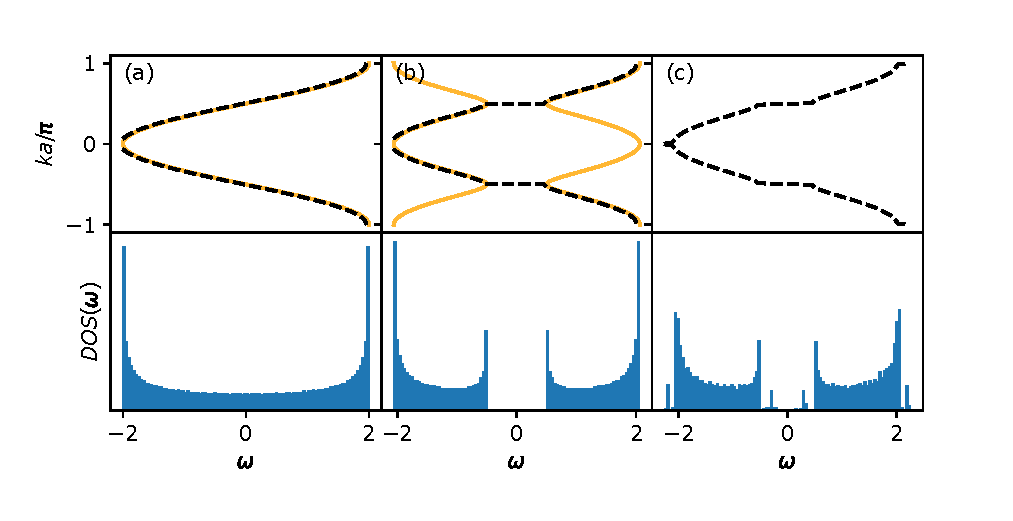
\includegraphics[width=1\textwidth,height=\textheight]{figure_code/background_chapter/simple_DOS}
\caption[{Cubic Lattice dispersion with disorder}]{The dispersion (upper row) and density of states (lower row) obtained from a cubic lattice model \(H = \sum_{i} V_i c^\dagger_{i}c_{i} - t \sum_{\langle i,j\rangle} c^\dagger_{i}c_{j}\) in one dimension. (a) With not external potential. (b) With a static charge density wave background \(V_i = (-1)^i\) (c) A static charge density wave background with 2\% binary disorder.}
\label{fig:simple_DOS}
\end{figure}
}

We will later add a long range interaction between the localised electrons so we will replace the immobile fermions with a classical Ising field \(S_i = 1 - 2d^\dagger_id_i = \pm\tfrac{1}{2}\).

\[\begin{aligned}
H_{\mathrm{FK}} = & \;U \sum_{i} S_i\;(c^\dagger_{i}c_{i} - \tfrac{1}{2}) -\;t \sum_{\langle i,j\rangle} c^\dagger_{i}c_{j}.\\ 
\end{aligned}\]

The FK model can be solved exaclty with dynamic mean field theory in the infinite dimensional~\autocite{antipovCriticalExponentsStrongly2014,ribicNonlocalCorrelationsSpectral2016,freericksExactDynamicalMeanfield2003,herrmannNonequilibriumDynamicalCluster2016}.

\begin{itemize}
\tightlist
\item
  displays disorder free localisation
\end{itemize}

\hypertarget{phase-diagrams}{%
\subsection{Phase Diagrams}\label{phase-diagrams}}

\hypertarget{fig:fk_phase_diagram}{%
\begin{figure}
\centering
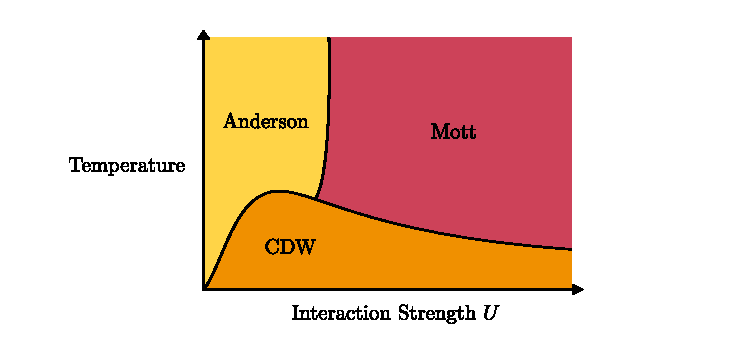
\includegraphics[width=1\textwidth,height=\textheight]{figure_code/background_chapter/fk_phase_diagram}
\caption[{Fermi-Hubbard and Falikov-Kimball Temperatue-Interaction Phase Diagrams}]{Schematic Phase diagrams of the Fermi-Hubbard (left) and Falikov-Kimball model (right) showing temperature (T) and repulsive interaction strength (U). Hubbard model diagram adapted from~\autocite{micnasSuperconductivityNarrowbandSystems1990}, Falikov-Kimball model from~\autocite{antipovInteractionTunedAndersonMott2016,antipovCriticalExponentsStrongly2014}}
\label{fig:fk_phase_diagram}
\end{figure}
}

\begin{itemize}
\tightlist
\item
  rich phase diagram in 2d Despite its simplicity, the FK model has a rich phase diagram in \(D \geq 2\) dimensions. For example, it shows an interaction-induced gap opening even at high temperatures, similar to the corresponding Hubbard Model~\autocite{brandtThermodynamicsCorrelationFunctions1989}.
\end{itemize}

At half filling and in dimensions greater than one, the FK model exhibits a phase transition at some \(U\) dependent critical temperature \(T_c(U)\) to a low temperature charge density wave state in which the spins order antiferromagnetically. This corresponds to the heavy electrons occupying one of the two sublattices A and B~\autocite{maskaThermodynamicsTwodimensionalFalicovKimball2006}. In the disordered region above \(T_c(U)\) there is a transition between an Anderson insulator phase at weak interaction and a Mott insulator phase in the strongly interacting regime~\autocite{andersonAbsenceDiffusionCertain1958}.

\begin{itemize}
\tightlist
\item
  superconductivity when doped
\end{itemize}

In 1D, the ground state phenomenology as the model is doped away from the half-filled state can be rich~\autocite{gruberGroundStatesSpinless1990} but the system is disordered for all \(T > 0\)~\autocite{kennedyItinerantElectronModel1986}.

In the one dimensional FK model there is no ordered CDW phase~\autocite{liebAbsenceMottTransition1968}. The supression of phase transition is a common phenomena in one dimensional systems. It can be understood via Peierls' argument~\autocite{peierlsIsingModelFerromagnetism1936,kennedyItinerantElectronModel1986} to be a consequence of the low energy penalty for domain walls in one dimensional systems.

Following Peierls' argument, consider the difference in free energy \(\Delta F = \Delta E - T\Delta S\) between an ordered state and a state with single domain wall in a discrete order parameter. Short range interactions produce a constant energy penalty for such a domain wall that does not scale with system size. In contrast, the number of such single domain wall states scales linearly so the entropy is \(\propto \ln L\). Thus the entropic contribution dominates (eventually) in the thermodynamic limit and no finite temperature order is possible. In two dimensions and above, the energy penalty of a domain wall scales like \(L^{d-1}\) so they can support ordered phases.

\hypertarget{long-ranged-ising-model}{%
\subsection{Long Ranged Ising model}\label{long-ranged-ising-model}}

Our extension to the FK model could now be though of as spinless fermions coupled to a long range Ising (LRI) model. The LRI model has been extensively studied and its behaviour may be bear relation to the behaviour of our modified FK model.

\[H_{\mathrm{LRI}} = \sum_{ij} J(|i-j|) \tau_i \tau_j = J \sum_{i\neq j} |i - j|^{-\alpha} \tau_i \tau_j\]

Renormalisation group analyses show that the LRI model has an ordered phase in 1D for \$1 \textless{} \alpha \textless{} 2 \$~\autocite{dysonExistencePhasetransitionOnedimensional1969}. Peierls' argument can be extended~\autocite{thoulessLongRangeOrderOneDimensional1969} to long range interactions to provide intuition for why this is the case. Again considering the energy difference between the ordered state \(|\ldots\uparrow\uparrow\uparrow\uparrow\ldots\rangle\) and a domain wall state \(|\ldots\uparrow\uparrow\downarrow\downarrow\ldots\rangle\). In the case of the LRI model, careful counting shows that this energy penalty is: \[\Delta E \propto \sum_{n=1}^{\infty} n J(n)\]

because each interaction between spins separated across the domain by a bond length \(n\) can be drawn between \(n\) equivalent pairs of sites. Ruelle proved rigorously for a very general class of 1D systems, that if \(\Delta E\) or its many-body generalisation converges in the thermodynamic limit then the free energy is analytic~\autocite{ruelleStatisticalMechanicsOnedimensional1968}. This rules out a finite order phase transition, though not one of the Kosterlitz-Thouless type. Dyson also proves this though with a slightly different condition on \(J(n)\)~\autocite{dysonExistencePhasetransitionOnedimensional1969}.

With a power law form for \(J(n)\), there are three cases to consider:

\$ \alpha = 0\$ For infinite range interactions the Ising model is exactly solveable and mean field theory is exact~\autocite{lipkinValidityManybodyApproximation1965}. This limit is the same as the infinite dimensional limit.

\$ \alpha \le 1\$ For slowly decaying interactions \(\sum_n J(n)\) does not converge so the Hamiltonian is non-extensive, a case which won't be further considered here. \textbf{cite}

\$ 1 \textless{} \alpha \textless{} 2 \$ A phase transition to an ordered state at a finite temperature.

\$ \alpha = 2 \$ The energy of domain walls diverges logarithmically, and this turns out to be a Kostelitz-Thouless transition~\autocite{thoulessLongRangeOrderOneDimensional1969}.

\$ 2 \textless{} \alpha \$ For quickly decaying interactions, domain walls have a finite energy penalty, hence Peirels' argument holds and there is no phase transition.

\hypertarget{fig:alpha_diagram}{%
\begin{figure}
\centering
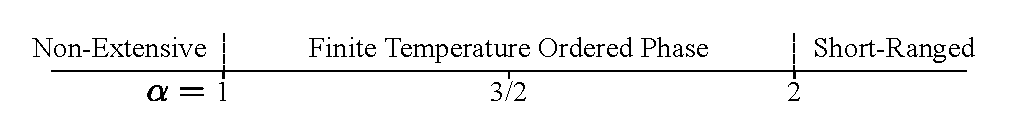
\includegraphics[width=1\textwidth,height=\textheight]{figure_code/background_chapter/alpha_diagram}
\caption[{Long Range Ising Model Behaviour}]{}
\label{fig:alpha_diagram}
\end{figure}
}

\begin{Shaded}
\begin{Highlighting}[]

\end{Highlighting}
\end{Shaded}
